\subsection{Children's polite speech understanding}
\label{sec:child}

Previously we have shown that adults in the US think about polite speech as reflecting a tradeoff between information transfer and face-saving. Will children reason similarly? Here we extend our tradeoff hypothesis to suggest that, starting at a young age, children distinguish between these goals and reason about the optimal degree of tradeoff (i.e. what is the nicest, most helpful thing to say) based on the speaker's intention, listener's need, and cultural expectations. Thus, adults and children should reason about polite language as broadly reflecting a tradeoff between information-saving and face-saving, although such understanding may mature over time. 

\subsubsection{Background}

There is not as much evidence for young children's understanding of polite speech (specifically white lies) as for children's production of polite speech. For example, children as young as 3 years start to tell white lies; they lie to the giver of an undesirable gift and say that the gift is nice \citep{talwar2007}. 

Interestingly, understanding of lies in general and motivations for white lies is displayed in later years than production: 8- and 11-, but not 4-year-olds, demonstrate correct categorization of truths as truths and lies as lies \citep{bussey1999}; 7- to 11-year-olds rate lies as more positive in politeness than transgression contexts \citep{heyman2009}. However, no study has yet looked at how children spontaneously reason about motivations behind lies and truths, especially those related to the epistemic-social tradeoff that we are currently interested in. 

\subsubsection{Empirical test: Experiment 3}

To examine my hypotheses about children's polite language understanding, I want to first look at how children start to reason about simple markers of politeness from a young age, when there is no conflict between goals (epistemic vs. social) and it is unambiguously better to be polite. Specifically, I predict that young children begin attributing simple intentions to be prosocial to speakers who use prominent markers of politeness (e.g. ``please,'' ``could you'') to make requests. 

\paragraph{Data collection procedure} Participants will be recruited at children's museum and nursery/elementary schools in US. I will recruit two different age groups (3- and 4-year-olds), with 24 participants per condition. Those who are not exposed to English at least 75\% daily will be excluded from data analysis. 

\paragraph{Design} I will vary the type of request made by the speaker: whether or not the request was polite (i.e. used ``please'' or ``can/could you~''; e.g. ``Could you please come to the store with me?'') or impolite (no polite marker; e.g. ``stop singing.'') Within the polite request, there will be variation on what kind of polite marker is used: (1) ``please''; (2) ``Can/could you'' (interrogative); and (3) ``Can/could you'' plus ``please.'' I will examine whether there are any differences in judgments for these varying polite syntactic forms. 

In each study session, I plan to present 12 different stories in which there are an impolite speaker (``Give me a cookie!'') and a polite speaker (``Can you please give me a cookie?''). I will then ask participants to indicate which speaker was nicer or more polite (vs. meaner or more rude), and ask about social implications of polite speech (preference: ``Who would you rather play with?'' and expected compliance: ``Who will get a cookie?''). 

\paragraph{Analysis plan} I will use a mixed-effects logistics regression model to analyze comparisons of polite vs. impolite speakers, as indicated by participants' indication of the speaker that: (1) was nicer/meaner/more polite/more rude; (2) is a preferred play partner; and (3) is more likely to gain compliance.

\subsubsection{Empirical test: Experiment 4}

After confirming that young children have a well-established understanding of polite speakers? prosocial intentions when there is no conflict in their goals, I want to look at how children reason about speakers who speak truthfully but impolitely, or politely but untruthfully. I propose a procedure that is based on the scenarios used with adults (Experiments P1 and P2), but simplified: participants will be asked to read a story in which, for example, two speakers tasted yucky cookies and were asked how they liked it, either by the baker himself, or someone else. One speaker speaks truthfully (``the cookie was yucky'') and the other untruthfully (``the cookie was tasty''). Participants will then judge whether each speaker was telling the truth and whether she was nice or mean, and indicate whether they prefer to play with the truthful speaker or the untruthful speaker. This procedure has been piloted and has worked well in India, as well as other two sites of interest (pilot findings are discussed in the next subsection).
 
{\bf Data collection procedure.} Participants will be recruited at children's museum and nursery/elementary schools in US. Across these three different sites, I will recruit three different age groups (3-4, 5-6, and 7-8-year-olds), with 24 participants per condition. Those who are not exposed to English at least 75\% daily will be excluded from data analysis. 

{\bf Design.} There are two independent variables: (1) listener type: whether or not the context was such that the `listeners' in our story asked about their own performance (e.g., cookie that they baked) or another, unknown person's performance (e.g., a cookie that was lying around for free); and (2) speaker type: whether the `speakers' in our story decide to tell a lie or truth about the performance. 

Each participant will be randomly assigned to one `listener' condition (i.e., whether the story is about listener's performance or someone else's) and will go through both `speaker' trials (i.e., speaker who tells a lie and speaker who tells the truth). Thus, the `listener' variable is a between-subjects, and the `speaker' variable is a within-subjects factor. There will be two sets of two speaker trials, and the order of the sets will be counterbalanced across subjects.

I will ask the following questions to participants: (1) In each trial, after telling the story of each speaker: ``Was [the speaker] in the story nice? Was she mean? Was she telling the truth?'' (the order of questions will be counterbalanced); (2) After one set of two trials, comparing two speakers, one who told a lie vs. one who told the truth: ``Who do you want to play with more, [polite speaker] or [honest speaker]?''

\begin{figure*}[t]
\begin{centering}
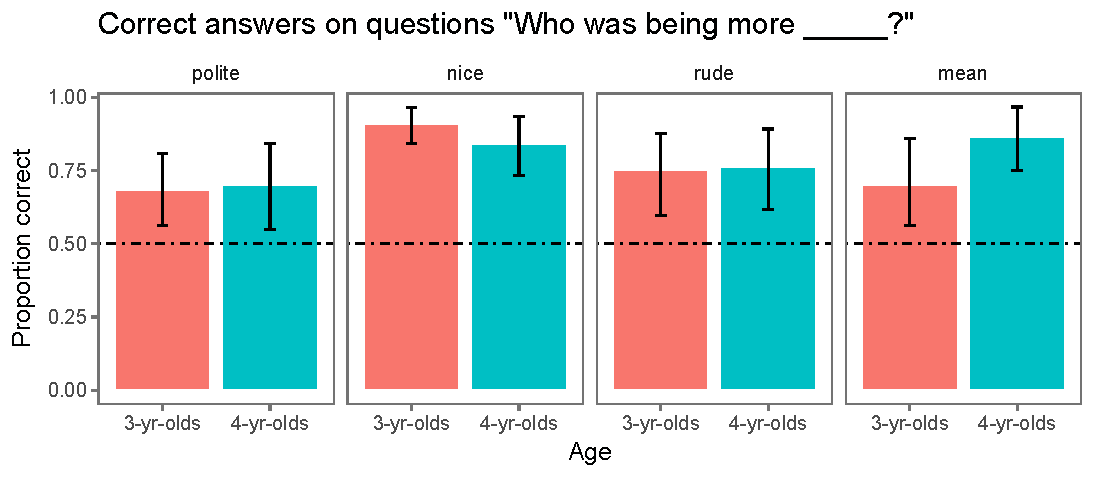
\includegraphics[width=\textwidth]{figures/youngchild.pdf}
\caption{\label{fig:expt3} Results from Experiment 3 (pilot), for children's judgments for polite vs. impolite speaker, when asked who was being nicer/meaner/more polite/more rude. Error bars represent 95\% confidence intervals.
}
\end{centering}
\end{figure*}


\begin{figure*}[h]
\begin{centering}
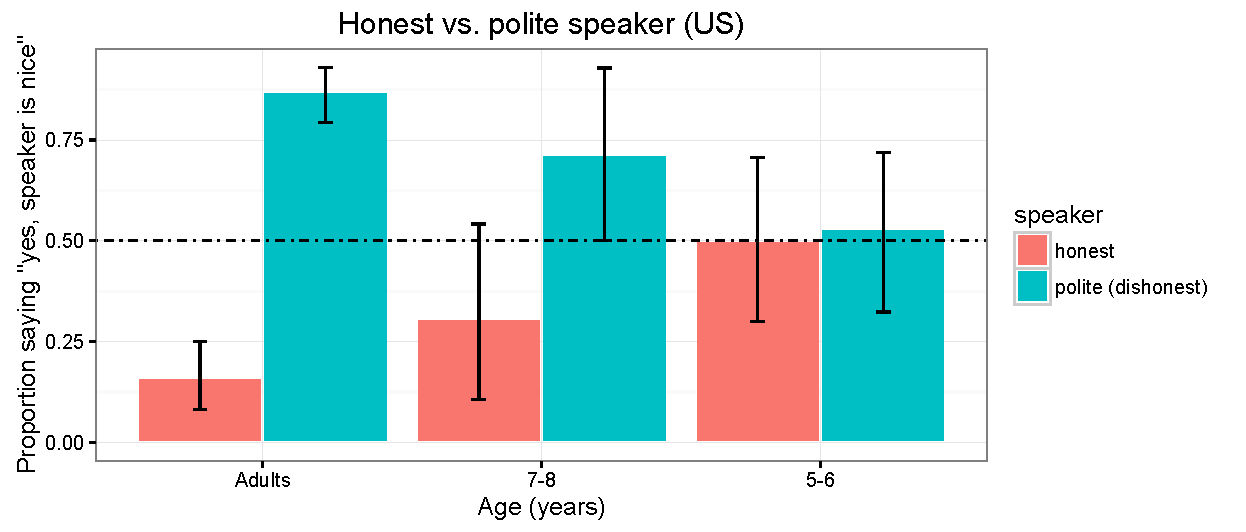
\includegraphics[width=\textwidth]{figures/exp3.pdf}
\caption{\label{fig:expt4} Results from Experiment 4 (pilot), for children's niceness judgment for honest versus polite (but dishonest) speaker. Error bars represent 95\% confidence intervals.}
\end{centering}
\end{figure*}




{\bf Analysis plan.} I will use a mixed-effects logistics regression model to analyze: (1) participants' rating for a given speaker's niceness/meanness/truth-telling; (2) comparisons of polite vs. honest speakers, as indicated by whom they ``want to play with.''

\subsubsection{Results from pilot work}

I have run pilot study of the two proposed experiments, and Figures~\ref{fig:expt3} and ~\ref{fig:expt4} are example analyses conducted on pilot data. 

Figure~\ref{fig:expt3} shows pilot results from Experiment 3, which indicate that 3- and 4-year-old children overall are able to judge correctly that a person who used polite markers such as ?please? and ?can you~? is more polite and nicer, whereas a person who failed to use such polite markers is more rude and meaner.

In Figure~\ref{fig:expt4} that shows pilot results from Experiment 4, an interesting developmental trend is seen where 8-year-olds show similar patterns of niceness attribution to adults but it is not as much differentiated between honest and polite speaker, whereas 6-year-olds do not differentiate between the honest and polite speaker at all.

\subsubsection{Implications for the model}

Pilot results for Experiment 3 seem to suggest that young children of 3-4 years of age already have the ability to understand speakers? prosocial intentions behind polite speech, when there is no conflict between informational and social goals. 

Based on the pilot results for Experiment 4, when epistemic and social goals conflict with each other, older children of 7-8 years seem to show similar patterns of inferences as adults for honest versus polite speakers, in that they judge polite speaker as nice and honest speaker as not nice. However,  5-6-year-olds do not seem to differentiate between the two speakers. Interpreting these results, if this pattern holds, is possible in two ways: younger children have the same mechanistic process for evaluating the epistemic-social tradeoff to determine the speaker's social utility, but this is obscured due to some cause such as task demand, or younger children do not see the utterance as reflecting the epistemic-social utility at all. The former would be in favor of our model and its universal application, but further evidence (with greater statistical power) is needed to assess the model fit to the data.


%%% Local Variables: 
%%% mode: latex
%%% TeX-master: "desc"
%%% End

